\documentclass[12pt]{beamer}
\usepackage{tabularx}

\title{Applications of Graph Theory and Probability
in the Board Game Ticket to Ride}
\author{R. Teal Witter \& Alex Lyford}
\institute{Middlebury College}
\date{January 16, 2020}

\begin{document}

\frame{\titlepage}

\begin{frame}{Ticket to Ride (USA)}
    \centering
    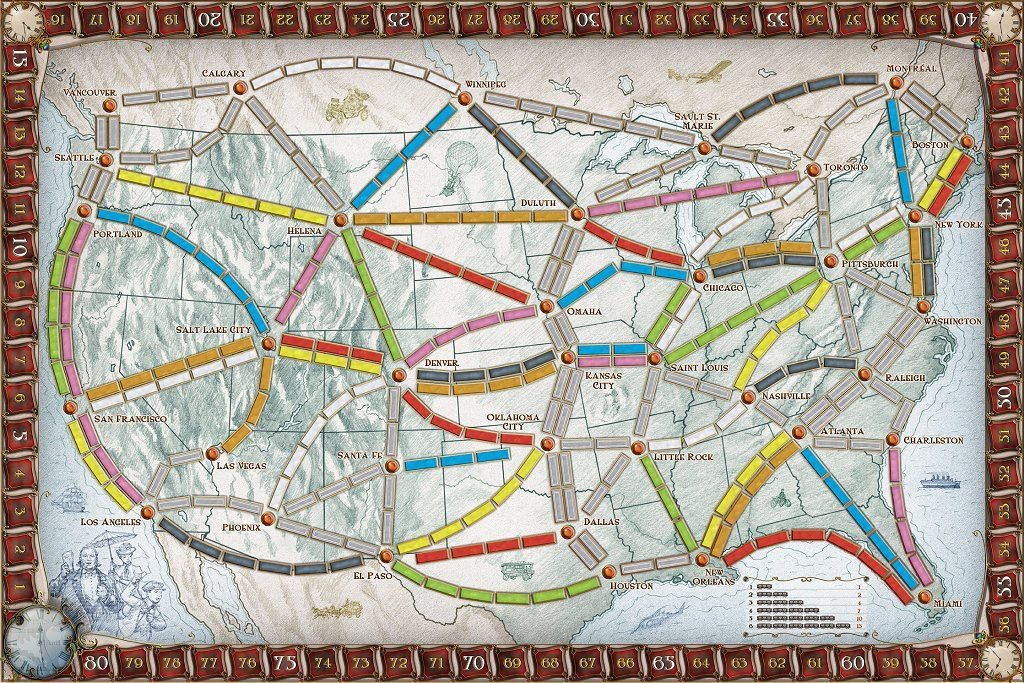
\includegraphics[scale=.3]{figures/board}
\end{frame}

\begin{frame}{Overview}
    \tableofcontents
\end{frame}

\section{Routes}

\begin{frame}{Current Route Values}
    \begin{center}
    \renewcommand{\arraystretch}{2}
    \begin{tabular}{| c | c | c | c | c | c | c |}
    \hline
     Route Length & 1 & 2 & 3 & 4 & 5 & 6\\
     \hline
     Points Scored & 1 & 2 & 4 & 7 & 10 & 15\\
     \hline
     Points per Train & 1.00 & 1.00 & $1.\overline{33}$ 
     & 1.75 & 2.00 & 2.50\\
     \hline
    \end{tabular}
    \end{center}
\end{frame}

\begin{frame}{Current Route Values: Why?}
    Explanation: 
    \begin{itemize}
    \item Collecting many trains of the same 
    color is hard\footnotemark
    \end{itemize}
    \vspace{.5cm}
    \pause
    Drawbacks: 
    \begin{itemize}
    \item Only one route can be purchased in each turn
    \item Is it really \textit{2.5} times harder per train to 
    collect six trains than one or two?
    \item Collecting trains for multiple routes 
    increases the likelihood \textit{some} desired 
    train appears each turn
    \end{itemize}
    \footnotetext[1]{How hard??}
\end{frame}

\begin{frame}{Games with Routes of Length at Most $k$}
    For all games, all 45 trains will be collected over 23 turns.\footnotemark[2]
    
    \vspace{.5cm}
    \renewcommand{\arraystretch}{1.5}
    \begin{tabular}{| c | c | c | c | c |}
    \hline
    $k$ & Composition & Points & Turns & Points per Turn\\
    \hline
    1 & 1 x 45 & 45 & 23 + 45 & 0.66\\
    \hline
    2 & 2 x 22, 1 x 1 & 45 & 23 + 23 & 0.98\\
    \hline
    3 & 3 x 15 & 60 & 23 + 15 & 1.58\\
    \hline
    4 & 4 x 11, 1 x 1 & 78 & 23 + 12 & 2.23\\
    \hline
    5 & 5 x 9 & 90 & 23 + 9 & 2.81\\
    \hline
    6 & 7 x 5, 5 x 2 & 95 & 23 + 7 & 3.17\\
    \hline
    \end{tabular}
    \footnotetext[2]{We ignore locomotives collected from the five face up cards.}
\end{frame}

\begin{frame}{Win Rate in Simulated Games}
\centering
\includegraphics[scale=.45]{"figures/win_rates"}
    
\end{frame}

\section{Destination Tickets}

\end{document}